Der folgende Abschnitt stellt drei reale Fallbeispiele vor.
\subsection{Quirky}
Quirky ist ein Unternehmen gegr�ndet von Ben Kaufman, welches in New York City angesiedelt ist. Die Gesch�ftsidee besteht darin eine �ffentlich zug�ngliche Onlineplattform einzurichten und �ber diese jedem einzelnen die M�glichkeit zu geben Produktideen vorzustellen(fr�her gegen eine Geb�hr). Andere User k�nnen nunmehr die Produktideen bewerten und Kommentieren. Kommen bei einer Produktidee gen�gend positive R�ckmeldungen wird das Produkt gemeinsam mit der Community entwickelt. Hier ist schon zu erkennen, dass die Community einen wichtigen Bestandteil des Unternehmens darstellt. Abbildung 1 zeigt den Einfluss der Community noch einmal grafisch. Um eine m�glichst starke Community aufzubauen ben�tigt es nat�rlich Anreize um die einzelnen User an das Unternehmen zu binden. Quirky verfolgt hier ma"sgeblich den monet�ren Ansatz und bietet laut einem Werbeslogan auf ihrer Website schon f�r einen Klick eine finanzielle Verg�tung.
\begin{figure}[h!]
	\caption{�bersicht �ber den Crowdsourcing-Prozess bei Quirky\cite{TENREASONSQUIRKY}}
	\centering
		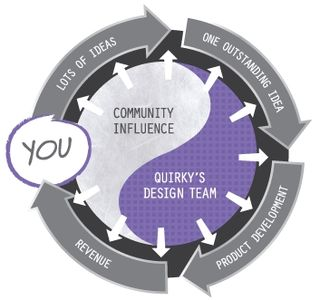
\includegraphics[scale=0.9]{figures/Quirky}
\end{figure}

Hierbei ist anzumerken, dass Quirky ein hybrides Modell an Community-Beteiligung und eigener Entwicklung nutzt. Quirky k�mmert sich um die Koordination sowie um die schwierigeren Entwicklungsschritte, wie zum Beispiel die technische Entwicklung des Produkts.

Quirky vertraut bei diesem Gesch�ftsmodell haupts�chlich auf die sogenannten Lead-User, welche in den vorangegangen Kapiteln genauer beschrieben wurden. Eine neue Idee einzureichen ist relativ einfach m�glich �ber die angebotene Online-Plattform(\url{www.quirky.com}). Es wird ein Titel, eine sogenannte \glqq Elevator Pitch\grqq (kurze Beschreibung des Produkts), eine Einteilung in eine von insgesamt 8 Kategorien, welches Problem die Idee l�st und wie das Problem gel�st werden kann.

Ein Nachteil der finanziellen Verg�tung in der Form wie sie Quirky anwendet, bei der man bei jeder Interaktion mit der Community Geld verdient ist, dass es zwar viele Interaktionen der Community gibt, jedoch die Qualit�t der Kommentare, Votings(man Voted f�r das bereits beste Produkt) fraglich ist. Quirky scheint dieses Problem jedoch nicht zu haben.

Ein weiteres Problem stellt die Abtretung der Rechte des Lead-Users dar, falls die Produktidee von Quirky angenommen wird. Es besteht zwar ein Anspruch auf eine entsprechende Verg�tung durch Quirky, jedoch wenn Patente angemeldet werden ist es fraglich wer als Erfinder eingetragen wird. Oftmals werden Produktideen von mehr als 800 Personen beeinflusst.
\cite{LOSINGRIGHTS}

Quirky hat mit Stand Dezember 2013 eine globale Community von 600000 Mitglieder, die Produkte entwerfen und beeinflussen.\cite{REPORTQUIRKY2345}


TODO 2 Seiten

\subsection{InnoCentive}
TODO

\subsection{Crowdspirit}
TODO fehlgeschlagene Crowdsourcing plattform